\runningheader{SAT Mathematics}{Drill Set 1}{Page \thepage\ of \numpages}

\begingradingrange{sat-drill-01}
\subsection*{SAT Drill 1} 

\question[1]
The total cost $f(x)$, in dollars, to lease a car for 36 months from a particular car dealership is given by $f(x) = 36x + 1,000$, where $x$ is the monthly payment, in dollars. What is the total cost to lease a car when the monthly payment is $\$400$?
\begin{choices}
  \choice $\$13,400$
  \choice $\$13,000$
  \CorrectChoice $\$15,400$
  \choice $\$37,400$
\end{choices}


\question[1]
A window repair specialist charges $\$220$ for the first two hours of repair plus an hourly fee for each additional hour. The total cost for 5 hours of repair is $\$400$. Which function $f$ gives the total cost, in dollars, for $x$ hours of repair, where $x \geq 2$?
\begin{choices}
  \CorrectChoice $f(x) = 60x + 100$
  \choice $f(x) = 60x + 220$
  \choice $f(x) = 80x$
  \choice $f(x) = 80x + 220$
\end{choices} 

\question[1]
The function $h$ is defined by $h(x) = 4x + 28$. The graph of $y = h(x)$ in the $xy$-plane has an $x$-intercept at $(a, 0)$ and a $y$-intercept at $(0, b)$, where $a$ and $b$ are constants. What is the value of $a + b$?
\begin{choices}
  \CorrectChoice 21
  \choice 28
  \choice 32
  \choice 35
\end{choices}

\newpage

\question[1]
An economist modeled the demand $Q$ for a certain product as a linear function of the selling price $P$. The demand was 20,000 units when the selling price was \$40 per unit, and the demand was 15,000 units when the selling price was $\$ 60$ per unit. Based on the model, what is the demand, in units, when the selling price is $\$ 55$ per unit?
\begin{choices}
  \CorrectChoice 16,250
  \choice 16,500
  \choice 16,750
  \choice 17,500
\end{choices}

\question[1]
The cost of renting a backhoe for up to 10 days is $\$ 270$ for the first day and $\$ 135$ for each additional day. Which of the following equations gives the cost $y$, in dollars, of renting the backhoe for $x$ days, where $x$ is a positive integer and $x \leq 10$?
\begin{choices}
  \choice $y = 270x - 135$
  \choice $y = 270x + 135$
  \choice $y = 135x + 270$
  \CorrectChoice $y = 135x + 135$
\end{choices}

\question[1]
The front of a roller-coaster car is at the bottom of a hill and is 15 feet above the ground. If the front of the roller-coaster car rises at a constant rate of 8 feet per second, which of the following equations gives the height $h$, in feet, of the front of the roller-coaster car $s$ seconds after it starts up the hill?
\begin{choices}
  \CorrectChoice $h = 8s + 15$
  \choice $h = 15s + \frac{335}{8}$
  \choice $h = 8s + \frac{335}{15}$
  \choice $h = 15s + 8$
\end{choices}

\newpage

\question[1]
According to a model, the head width, in millimeters, of a worker bumblebee can be estimated by adding 0.6 to four times the body weight of the bee, in grams. According to the model, what would be the head width, in millimeters, of a worker bumblebee that has a body weight of 0.5 grams?
\begin{solutionorbox}
$2.6$
\end{solutionorbox}


\question[1]
If $f$ is the function defined by $f(x) = \frac{2x-1}{3}$, what is the value of $f(5)$?
\begin{choices}
  \choice $\frac{4}{3}$
  \choice $\frac{7}{3}$
  \CorrectChoice 3
  \choice 9
\end{choices}

\question[1]
$$
d = 16t
$$
The given equation represents the distance $d$, in inches, where $t$ represents the number of seconds since an object started moving. Which of the following is the best interpretation of 16 in this context?
\begin{choices}
  \choice The object moved a total of 16 inches.
  \choice The object moved a total of $16t$ inches.
  \CorrectChoice The object is moving at a rate of 16 inches per second.
  \choice The object is moving at a rate of $\frac{1}{16}$ inches per second.
\end{choices}

\newpage


\question[1]
{\raggedright For the given linear function $f$, which table gives three values of $x$ and their corresponding values of $f(x)$?\par}
\vspace{0.5em}
\begin{oneparchoices}
  \choice \parbox[t][1.35in][t]{0.38\linewidth}{\centering
    \begin{tabular}{|c|c|}
    \hline
    $x$ & $f(x)$ \\
    \hline
    0 & 0 \\
    \hline
    1 & 0 \\
    \hline
    2 & 0 \\
    \hline
    \end{tabular}}
  \choice \parbox[t][1.35in][t]{0.38\linewidth}{\centering
    \begin{tabular}{|c|c|}
    \hline
    $x$ & $f(x)$ \\
    \hline
    0 & 39 \\
    \hline
    1 & 39 \\
    \hline
    2 & 39 \\
    \hline
    \end{tabular}}
  \CorrectChoice \parbox[t][1.35in][t]{0.38\linewidth}{\centering
    \begin{tabular}{|c|c|}
    \hline
    $x$ & $f(x)$ \\
    \hline
    0 & 0 \\
    \hline
    1 & 39 \\
    \hline
    2 & 78 \\
    \hline
    \end{tabular}}
  \choice \parbox[t][1.35in][t]{0.38\linewidth}{\centering
    \begin{tabular}{|c|c|}
    \hline
    $x$ & $f(x)$ \\
    \hline
    0 & 39 \\
    \hline
    1 & 0 \\
    \hline
    2 & -39 \\
    \hline
    \end{tabular}}
\end{oneparchoices}

\question[1]
Hector used a tool called an auger to remove corn from a storage bin at a constant rate. The bin contained 24,000 bushels of corn when Hector began to use the auger. After 5 hours of using the auger, 19,350 bushels of corn remained in the bin. If the auger continues to remove corn at this rate, what is the total number of hours Hector will have been using the auger when 12,840 bushels of corn remain in the bin?
\begin{choices}
  \choice 3
  \choice 7
  \CorrectChoice 8
  \choice 12
\end{choices}

\question[1]
What value of $p$ satisfies the equation $5p + 180 = 250$?
\begin{choices}
  \CorrectChoice 14
  \choice 65
  \choice 86
  \choice 250
\end{choices}

\newpage 


\question[1]
$$
4x + 5 = 165
$$
What is the solution to the given equation?
\begin{solutionorbox}
$x=40$
\end{solutionorbox}

\question[1]
John paid a total of $\$ 165$ for a microscope by making a down payment of $\$ 37$ plus $p$ monthly payments of $\$ 16$ each. Which of the following equations represents this situation?
\begin{choices}
  \choice $16p - 37 = 165$
  \choice $37p - 16 = 165$
  \CorrectChoice $16p + 37 = 165$
  \choice $37p + 16 = 165$
\end{choices}

\question[1]
$$
3x + 21 = 3x + k
$$
In the given equation, $k$ is a constant. The equation has infinitely many solutions. What is the value of $k$?
\begin{solutionorbox}
$k=21$
\end{solutionorbox}

\newpage

\question[1]
$3(2x - 6) - 11 = 4(x - 3) + 6$

If $x$ is the solution to the equation above, what is the value of $x - 3$?
\begin{choices}
  \choice $\frac{23}{2}$
  \CorrectChoice $\frac{17}{2}$
  \choice $\frac{15}{2}$
  \choice $-\frac{15}{2}$
\end{choices}

\question[1]
Alan drives an average of 100 miles each week. His car can travel an average of 25 miles per gallon of gasoline. Alan would like to reduce his weekly expenditure on gasoline by $\$ 5$. Assuming gasoline costs $\$ 4$ per gallon, which equation can Alan use to determine how many fewer average miles, $m$, he should drive each week?
\begin{choices}
  \choice $\frac{25}{4}m = 95$
  \choice $\frac{25}{4}m = 5$
  \choice $\frac{4}{25}m = 95$
  \CorrectChoice $\frac{4}{25}m = 5$
\end{choices}

\question[1]
$$
2n + 6 = 14
$$
A tree had a height of 6 feet when it was planted. The equation above can be used to find how many years $n$ it took the tree to reach a height of 14 feet. Which of the following is the best interpretation of the number 2 in this context?
\begin{choices}
  \choice The number of years it took the tree to double its height
  \CorrectChoice The average number of feet that the tree grew per year
  \choice The height, in feet, of the tree when the tree was 1 year old
  \choice The average number of years it takes similar trees to grow 14 feet
\end{choices}

\newpage

\question[1]
$$
2x + 16 = a(x + 8)
$$
In the given equation, $a$ is a constant. If the equation has infinitely many solutions, what is the value of $a$?
\begin{solutionorbox}
$2$
\end{solutionorbox}

\question[1]
If $\frac{x}{8} = 5$, what is the value of $\frac{8}{x}$?
\begin{solutionorbox}
$\frac{1}{5}$
\end{solutionorbox}


\question[1]
\phantom{\space}\\
\begin{center}
\begin{tabular}{|c|c|}
\hline
$x$ & $y$ \\
\hline
18 & 130 \\
\hline
23 & 160 \\
\hline
26 & 178 \\
\hline
\end{tabular}
\end{center}
For line $h$, the table shows three values of $x$ and their 
corresponding values of $y$. Line $k$ is the result of translating 
line $h$ down 5 units in the $xy$-plane. What is the $x$-intercept of line $k$?
\begin{choices}
  \choice $\left(-\frac{26}{3}, 0\right)$
  \choice $\left(-\frac{9}{2}, 0\right)$
  \choice $\left(-\frac{11}{3}, 0\right)$
  \CorrectChoice $\left(-\frac{17}{6}, 0\right)$
\end{choices}

\newpage


\question[1]
\phantom{\space}\\
\begin{center}
\begin{tabular}{|c|c|}
\hline
$x$ & $y$ \\
\hline
$k$ & 13 \\
\hline
$k+7$ & -15 \\
\hline
\end{tabular}
\end{center}

The table gives the coordinates of two points on a line in the $xy$-plane. The $y$-intercept of the line is $(k-5, b)$, where $k$ and $b$ are constants. What is the value of $b$?
\begin{solutionorbox}
$33$
\end{solutionorbox}


\question[1]
Line $k$ is defined by $y = -\frac{17}{3}x + 5$. Line $j$ is perpendicular to line $k$ in the $xy$-plane. What is the slope of line $j$?
\begin{solutionorbox}
$\frac{3}{17}$
\end{solutionorbox}


\question[1]
The graph of the equation $ax + ky = 6$ is a line in the $xy$-plane, where $a$ and $k$ are constants. If the line contains the points $(-2, -6)$ and $(0, -3)$, what is the value of $k$?
\begin{choices}
  \CorrectChoice -2
  \choice -1
  \choice 2
  \choice 3
\end{choices}

\newpage


\question[1]
A certain apprentice has enrolled in 85 hours of training courses. The equation $10x + 15y = 85$ represents this situation, where $x$ is the number of on-site training courses and $y$ is the number of online training courses this apprentice has enrolled in. How many more hours does each online training course take than each on-site training course?
\begin{solutionorbox}
$5$ hours
\end{solutionorbox}

\question[1]
A store sells two different-sized containers of a certain Greek yogurt. The store's sales of this Greek yogurt totaled $1,277.94$ dollars last month. The equation $5.48x + 7.30y = 1,277.94$ represents this situation, where $x$ is the number of smaller containers sold and $y$ is the number of larger containers sold. According to the equation, which of the following represents the price, in dollars, of each smaller container?
\begin{choices}
  \CorrectChoice 5.48
  \choice $7.30y$
  \choice 7.30
  \choice $5.48x$
\end{choices}


\question[1]
Line $k$ is defined by $y = 3x + 15$. Line $j$ is perpendicular to line $k$ in the $xy$-plane. What is the slope of line $j$?
\begin{choices}
  \CorrectChoice $-\frac{1}{3}$
  \choice $-\frac{1}{12}$
  \choice $-\frac{1}{18}$
  \choice $-\frac{1}{45}$
\end{choices}


\newpage



\question[1]
Line $p$ is defined by $4y + 8x = 6$. Line $r$ is perpendicular to line $p$ in the $xy$-plane. What is the slope of line $r$?
\begin{solutionorbox}
$\frac{1}{2}$
\end{solutionorbox}

\question[1]
Line $p$ is defined by $2y + 18x = 9$. Line $r$ is perpendicular to line $p$ in the $xy$-plane. What is the slope of line $r$?
\begin{choices}
  \choice -9
  \choice $-\frac{1}{9}$
  \CorrectChoice $\frac{1}{9}$
  \choice 9
\end{choices}

\question[1]
$$y=x+4$$
Which table gives three values of $x$ and their corresponding values of $y$ for the given equation?
\phantom{\space}\\
\begin{oneparchoices}
  \CorrectChoice \parbox[t][1.35in][t]{0.38\linewidth}{\centering
    \begin{tabular}{|c|c|}
    \hline
    $x$ & $y$ \\
    \hline
    0 & 4 \\
    \hline
    1 & 5 \\
    \hline
    2 & 6 \\
    \hline
    \end{tabular}}
  \choice \parbox[t][1.35in][t]{0.38\linewidth}{\centering
    \begin{tabular}{|c|c|}
    \hline
    $x$ & $y$ \\
    \hline
    0 & 6 \\
    \hline
    1 & 5 \\
    \hline
    2 & 4 \\
    \hline
    \end{tabular}}
  \choice \parbox[t][1.35in][t]{0.38\linewidth}{\centering
    \begin{tabular}{|c|c|}
    \hline
    $x$ & $y$ \\
    \hline
    0 & 2 \\
    \hline
    1 & 1 \\
    \hline
    2 & 0 \\
    \hline
    \end{tabular}}
  \choice \parbox[t][1.35in][t]{0.38\linewidth}{\centering
    \begin{tabular}{|c|c|}
    \hline
    $x$ & $y$ \\
    \hline
    0 & 0 \\
    \hline
    1 & 1 \\
    \hline
    2 & 2 \\
    \hline
    \end{tabular}}
\end{oneparchoices}

\newpage



\question[1]
A cargo helicopter delivers only 100-pound packages and 120-pound packages. For each delivery trip, the helicopter must carry at least 10 packages, and the total weight of the packages can be at most 1,100 pounds. What is the maximum number of 120-pound packages that the helicopter can carry per trip?
\begin{choices}
  \choice 2
  \choice 4
  \choice 5
  \CorrectChoice 6
\end{choices}

\question[1]
The point $(8,2)$ in the $xy$-plane is a solution to which of the following systems of inequalities?
\begin{choices}
  \CorrectChoice $x > 0,\ y > 0$
  \choice $x > 0,\ y < 0$
  \choice $x < 0,\ y > 0$
  \choice $x < 0,\ y < 0$
\end{choices}



\question[1]
Adam's school is a 20-minute walk or a 5-minute bus ride away from his house. The bus runs once every 30 minutes, and the number of minutes, $w$, that Adam waits for the bus varies between 0 and 30. Which of the following inequalities gives the values of $w$ for which it would be faster for Adam to walk to school?
\begin{choices}
  \choice $w - 5 < 20$
  \choice $w - 5 > 20$
  \choice $w + 5 < 20$
  \CorrectChoice $w + 5 > 20$
\end{choices}

\newpage

\question[1]
Marisa needs to hire at least 10 staff members for an upcoming project. The staff members will be made up of junior directors, who will be paid $\$ 640$ per week, and senior directors, who will be paid $\$ 880$ per week. Her budget for paying the staff members is no more than $\$ 9,700$ per week. She must hire at least 3 junior directors and at least 1 senior director. Which of the following systems of inequalities represents the conditions described if $x$ is the number of junior directors and $y$ is the number of senior directors?
\begin{choices}
  \choice $640x + 880y \geq 9,\!700$, $x + y \leq 10$, $x \geq 3$, $y \geq 1$
  \CorrectChoice $640x + 880y \leq 9,\!700$, $x + y \geq 10$, $x \geq 3$, $y \geq 1$
  \choice $640x + 880y \geq 9,\!700$, $x + y \geq 10$, $x \leq 3$, $y \leq 1$
  \choice $640x + 880y \leq 9,\!700$, $x + y \leq 10$, $x \leq 3$, $y \leq 1$
\end{choices}


\question[1]
Valentina bought two containers of beads. In the first container 30\% of the beads are red, and in the second container $70 \%$ of the beads are red. Together, the containers have at least 400 red beads. Which inequality shows this relationship, where $x$ is the total number of beads in the first container and $y$ is the total number of beads in the second container?
\begin{choices}
  \CorrectChoice $0.3x + 0.7y \geq 400$
  \choice $0.7x + 0.3y \leq 400$
  \choice $\frac{x}{3} + \frac{y}{7} \leq 400$
  \choice $30x + 70y \geq 400$
\end{choices}


\newpage


\question[1]
The total cost, in dollars, to rent a surfboard consists of a $\$ 25$ service fee and a $\$ 10$ per hour rental fee. A person rents a surfboard for $t$ hours and intends to spend a maximum of $\$ 75$ to rent the surfboard. Which inequality represents this situation?
\begin{choices}
  \choice $10t \leq 75$
  \choice $10 + 25t \leq 75$
  \choice $25t \leq 75$
  \CorrectChoice $25 + 10t \leq 75$
\end{choices}

\question[1]
In North America, the standard width of a parking space is at least 7.5 feet and no more than 9.0 feet. A restaurant owner recently resurfaced the restaurant's parking lot and wants to determine the number of parking spaces, $n$, in the parking lot that could be placed perpendicular to a curb that is 135 feet long, based on the standard width of a parking space. Which of the following describes all the possible values of $n$?
\begin{choices}
  \choice $18 \leq n \leq 135$
  \choice $7.5 \leq n \leq 9$
  \choice $15 \leq n \leq 135$
  \CorrectChoice $15 \leq n \leq 18$
\end{choices}



\question[1]
$$
\begin{aligned}
& y \leq x \\
& y \leq -x
\end{aligned}
$$

Which of the following ordered pairs $(x, y)$ is a solution to the system of inequalities above?
\begin{choices}
  \choice $(1,0)$
  \choice $(-1,0)$
  \choice $(0,1)$
  \CorrectChoice $(0,-1)$
\end{choices}


\newpage

\question[1]
A laundry service is buying detergent and fabric softener from its supplier. The supplier will deliver no more than 300 pounds in a shipment. Each container of detergent weighs 7.35 pounds, and each container of fabric softener weighs 6.2 pounds. The service wants to buy at least twice as many containers of detergent as containers of fabric softener. Let $d$ represent the number of containers of detergent, and let $s$ represent the number of containers of fabric softener, where $d$ and $s$ are nonnegative integers. Which of the following systems of inequalities best represents this situation?
\begin{choices}
  \CorrectChoice $7.35d + 6.2s \leq 300,\ d \geq 2s$
  \choice $7.35d + 6.2s \leq 300,\ d \leq 2s$
  \choice $7.35d + 6.2s \geq 300,\ d \geq 2s$
  \choice $7.35d + 6.2s \geq 300,\ d \leq 2s$
\end{choices}


\question[1]
On a car trip, Rhett and Jessica each drove for part of the trip, and the total distance they drove was under 220 miles. Rhett drove at an average speed of 35 miles per hour (mph), and Jessica drove at an average speed of 40 mph. Which of the following inequalities represents this situation, where $r$ is the number of hours Rhett drove and $j$ is the number of hours Jessica drove?
\begin{choices}
  \choice $35r + 40j > 220$
  \CorrectChoice $35r + 40j < 220$
  \choice $40r + 35j > 220$
  \choice $40r + 35j < 220$
\end{choices}

\newpage

\question[1]
\begin{align*}
  -x + y &= -3.5 \\
  x + 3y &= 9.5
\end{align*}
If $(x, y)$ satisfies the system of equations above, what is the value of $y$?
\begin{solutionorbox}
$\frac{3}{2}$
\end{solutionorbox}

\question[1]
\[
\begin{aligned}
\frac{1}{2}y &= 4 \\
x - \frac{1}{2}y &= 2
\end{aligned}
\]
The system of equations above has solution ($x$, $y$). What is the value of $x$?
\begin{choices}
  \choice 3
  \choice $\frac{7}{2}$
  \choice 4
  \CorrectChoice 6
\end{choices}



\question[1]
$$
\begin{gathered}
5x = 15 \\
-4x + y = -2
\end{gathered}
$$
The solution to the given system of equations is $(x, y)$. What is the value of $x + y$?
\begin{choices}
  \choice -17
  \choice -13
  \CorrectChoice 13
  \choice 17
\end{choices}


\newpage

\question[1]
$$
\begin{gathered}
\frac{3}{2}y - \frac{1}{4}x = \frac{2}{3} - \frac{3}{2}y \\
\frac{1}{2}x + \frac{3}{2} = py + \frac{9}{2}
\end{gathered}
$$

In the given system of equations, $p$ is a constant. If the system has no solution, what is the value of $p$?
\begin{solutionorbox}
$6$
\end{solutionorbox}

\question[1]
Hiro and Sofia purchased shirts and pants from a store. The price of each shirt purchased was the same and the price of each pair of pants purchased was the same. Hiro purchased 4 shirts and 2 pairs of pants for $\$ 86$, and Sofia purchased 3 shirts and 5 pairs of pants for $\$ 166$. Which of the following systems of linear equations represents the situation, if $x$ represents the price, in dollars, of each shirt and $y$ represents the price, in dollars, of each pair of pants?
\begin{choices}
  \CorrectChoice
  $4x + 2y = 86$, $3x + 5y = 166$
  \choice
  $4x + 3y = 86$, $2x + 5y = 166$
  \choice
  $4x + 2y = 166$, $3x + 5y = 86$
  \choice
  $4x + 3y = 166$, $2x + 5y = 86$
\end{choices}


\newpage

\question[1]
\phantom{\space}\\
\begin{center}
  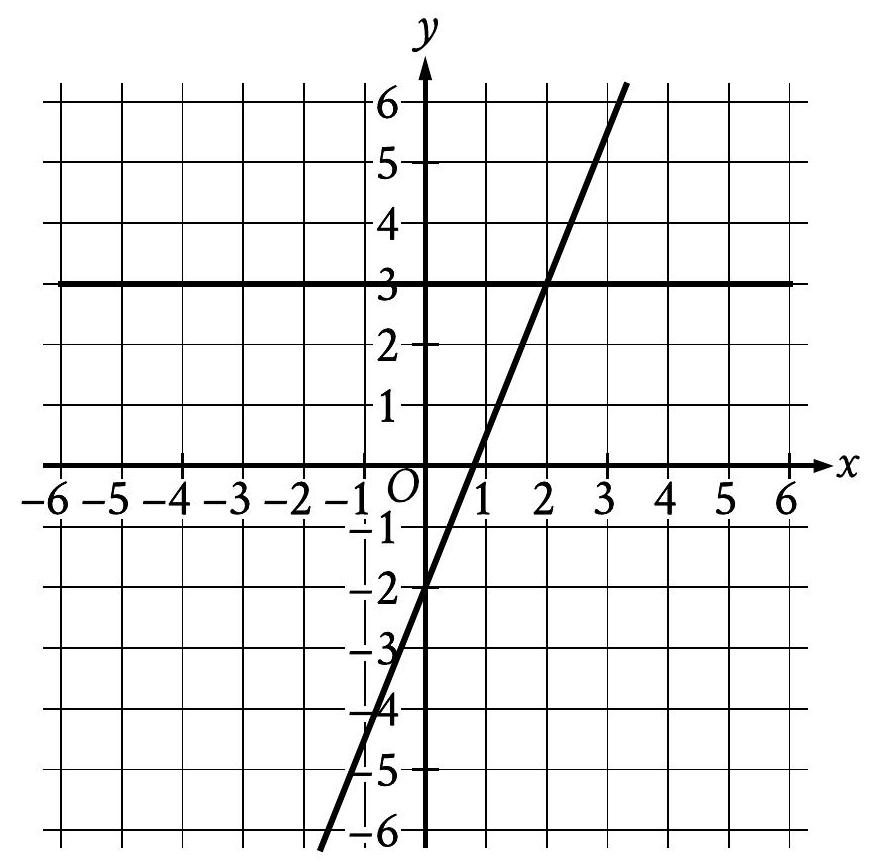
\includegraphics[width=0.80\linewidth]{images/2025_06_15_7d5ca6a095740ea44a32g-06}
\end{center}
The graph of a system of linear equations is shown. What is the solution $(x, y)$ to the system?
\begin{choices}
  \choice $(0,3)$
  \choice $(1,3)$
  \CorrectChoice $(2,3)$
  \choice $(3,3)$
\end{choices}

\question[1]
A company that provides whale-watching tours takes groups of 21 people at a time. The company's revenue is 80 dollars per adult and 60 dollars per child. If the company's revenue for one group consisting of adults and children was 1,440 dollars, how many people in the group were children?
\begin{choices}
  \choice 3
  \choice 9
  \CorrectChoice 12
  \choice 18
\end{choices}

\newpage 

\question[1]
At how many points do the graphs of the equations $y = x + 20$ and $y = 8x$ intersect in the $xy$-plane?
\begin{choices}
  \choice 0
  \CorrectChoice 1
  \choice 2
  \choice 8
\end{choices}

\question[1]
$$
\begin{gathered}
y = 3x \\
2x + y = 12
\end{gathered}
$$

The solution to the given system of equations is $(x, y)$. What is the value of $5x$?
\begin{choices}
  \choice 24
  \choice 15
  \CorrectChoice 12
  \choice 5
\end{choices}

\question[1]
A group of 202 people went on an overnight camping trip, taking 60 tents with them. Some of the tents held 2 people each, and the rest held 4 people each. Assuming all the tents were filled to capacity and every person got to sleep in a tent, exactly how many of the tents were 2-person tents?
\begin{choices}
  \choice 30
  \choice 20
  \CorrectChoice 19
  \choice 18
\end{choices}


\endgradingrange{sat-drill-01}